
\item Quando o cilindro de \SI{50}{\kilogram} é solto do repouso, a mola é submetida a uma tração de \SI{60}{\newton}. Determine a velocidade do cilindro após ele ter caído \SI{200}{\milli\meter}. Qual é a distância que ele caiu antes de parar instantaneamente?

\import{answers/}{answer-11}

\vspace{3cm}
\begin{flushleft}
	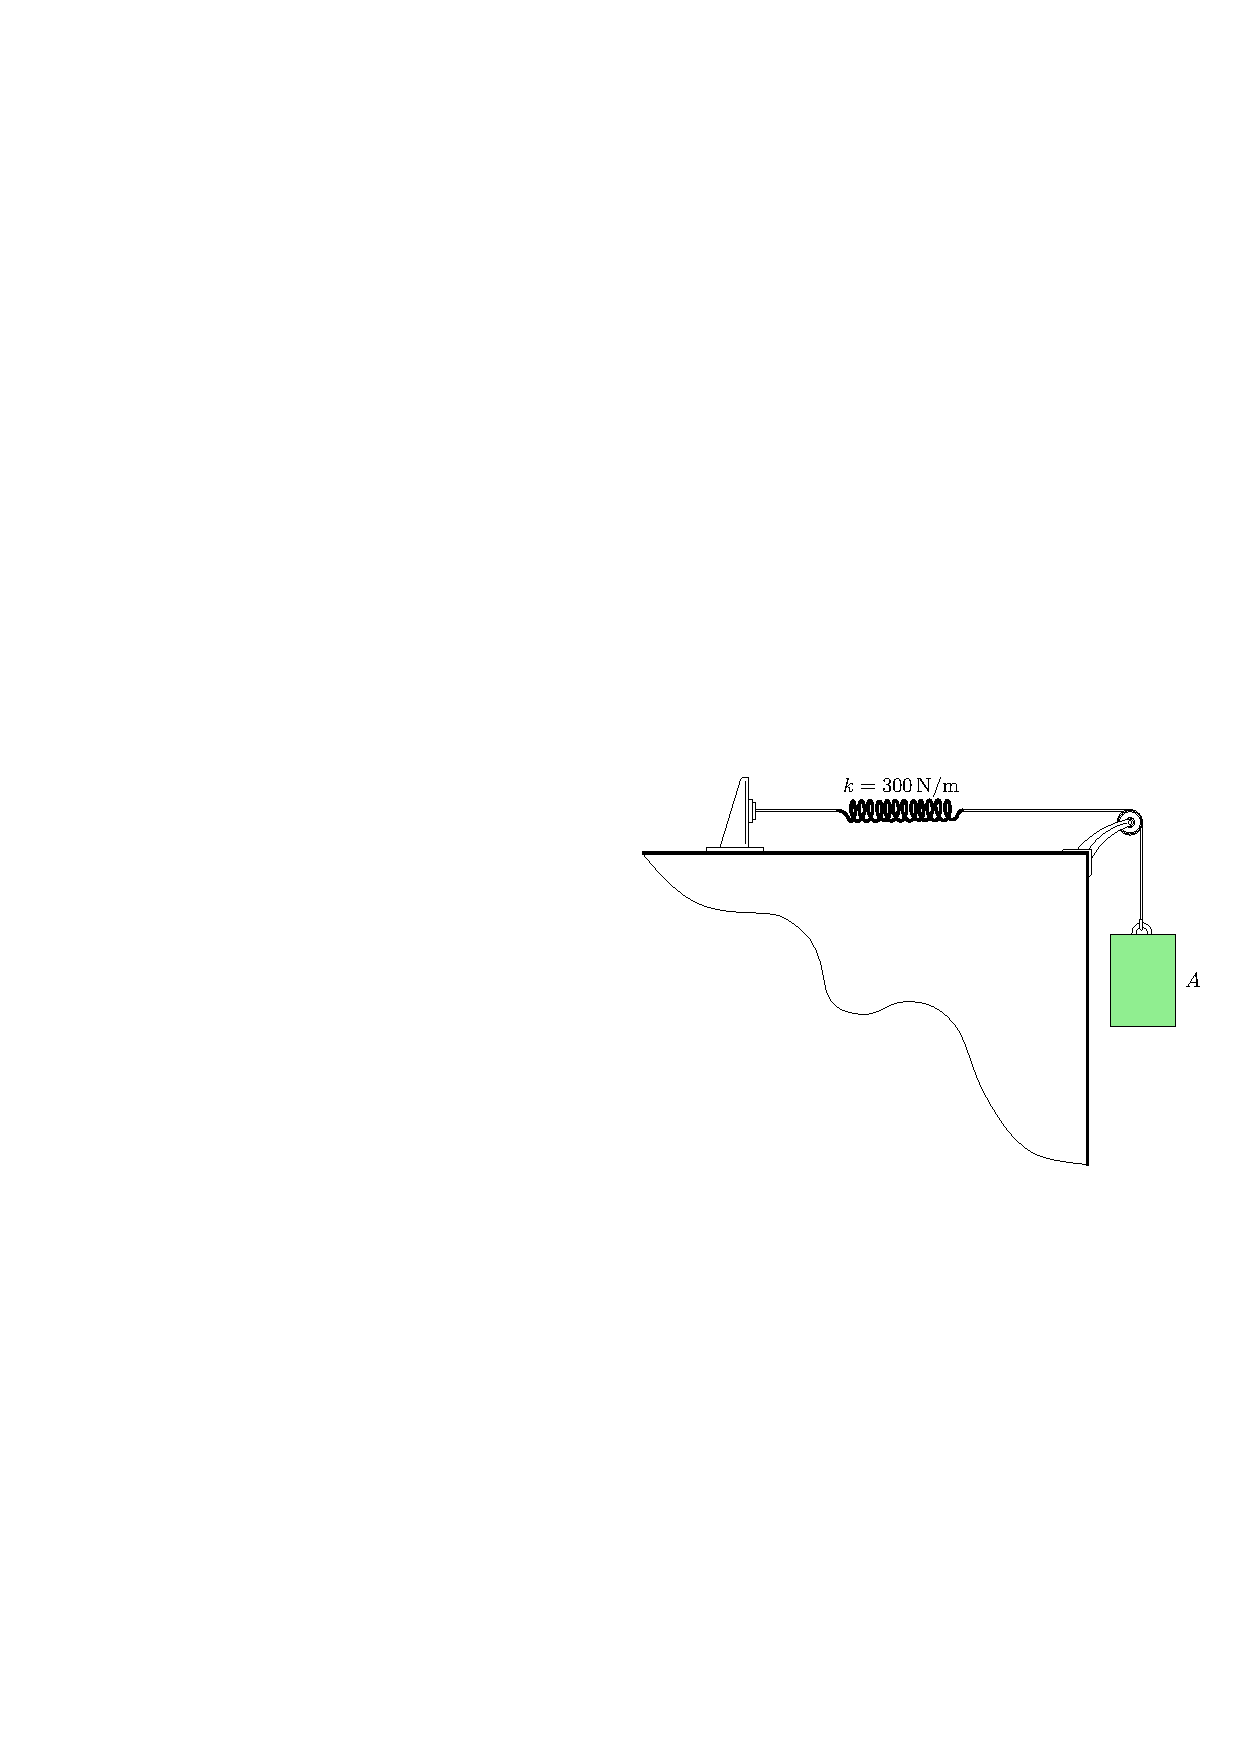
\includegraphics[scale=1.3]{images/draw_11.pdf}
\end{flushleft}